\subsection{Model Comparison and Internal Validation}

We compared the renewed primary Bayesian joint longitudinal--interval model with four prespecified alternatives: a descriptive Kaplan--Meier curve based on first observed DMR visit time, a discrete-time interval model with timing and visit-gap terms but no longitudinal MRD, a landmark MRD model using the last observed MRD before 6-, 12-, or 18-month landmarks, and a joint model that treated assay-floor observations as exact values at \(-5.0\). The Kaplan--Meier analysis was retained only as a descriptive benchmark because true DMR onset was interval-observed.

\begin{table}[!htbp]
\centering
\caption{Model comparison and internal validation. Event counts are shown as evaluated records/events. Validated Brier scores are patient-cluster bootstrap optimism-corrected for refittable simpler models; for the two Stan joint models, they are fixed-posterior bootstrap summaries without Stan refitting.}
\label{tab:model-comparison-validation}
\resizebox{\linewidth}{!}{%
\begin{tabular}{lrrrrrrll}
\toprule
Model & Interval n/events & Interval Brier & Validated interval Brier & Patient n/events & Patient Brier & Validated patient Brier & Interval cal. int./slope & Patient cal. int./slope \\
\midrule
Descriptive Kaplan--Meier & 275/68 & 0.172 & 0.182 & 87/68 & 0.362 & 0.370 & 0.497/0.433 & 2.059/-0.124 \\
Interval timing + visit gap & 275/68 & 0.174 & 0.178 & 87/68 & 0.290 & 0.296 & 0.000/1.000 & 1.271/-0.345 \\
Landmark MRD & 55/20 & 0.211 & 0.246 & 32/20 & 0.267 & 0.303 & -0.000/1.000 & 0.756/0.387 \\
Joint model, floor exact & 275/68 & 0.094 & 0.094 & 87/68 & 0.123 & 0.123 & -0.008/1.617 & 1.360/2.419 \\
Primary joint model & 275/68 & 0.082 & 0.082 & 87/68 & 0.116 & 0.116 & 0.003/1.784 & 1.329/2.816 \\
\bottomrule
\end{tabular}
}%
\end{table}



The descriptive Kaplan--Meier benchmark had interval-level Brier score 0.172 and patient-level Brier score 0.362. The interval timing--gap model improved interval-level calibration by directly modeling at-risk intervals, with interval Brier score 0.174 and optimism-corrected interval Brier score 0.178. The landmark MRD model was clinically interpretable but evaluable only among intervals with a prior landmark MRD measurement and patients still at risk; therefore, its performance is not directly comparable with full-cohort models.

The exact-floor joint model and the left-censored primary joint model had similar interval-level discrimination and calibration summaries, but the primary model is statistically preferable because it respects the assay reporting mechanism. Treating floor observations as exact \(-5.0\) values imposes artificial precision at the deepest molecular response levels, whereas the primary model contributes the likelihood probability \(P(y\leq -5.0)\). The primary model had interval Brier score 0.082 and patient-level Brier score 0.116; the corresponding exact-floor values were 0.094 and 0.123.

\begin{figure}[!htbp]
\centering
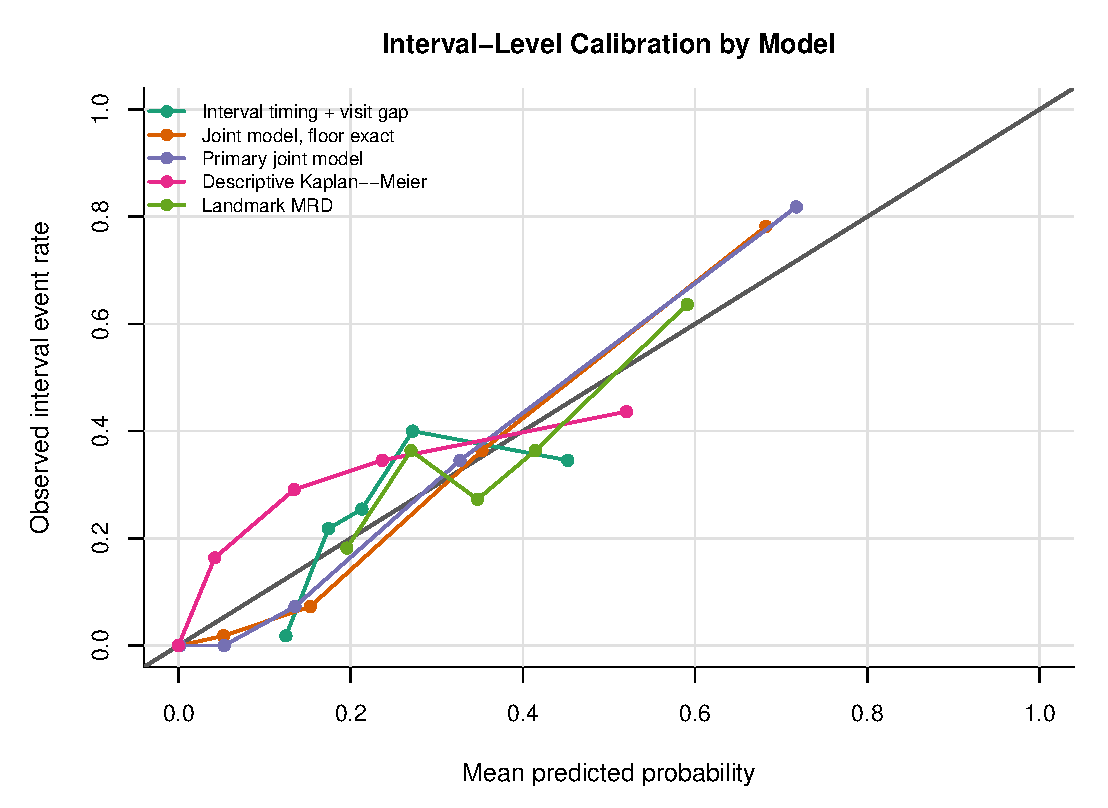
\includegraphics[width=0.82\linewidth]{figure_10_model_comparison_interval_calibration.pdf}
\caption{Interval-level observed-versus-predicted calibration across model classes. The Kaplan--Meier curve is descriptive because it uses first observed DMR visit time.}
\label{fig:model-comparison-interval-calibration}
\end{figure}

\begin{figure}[!htbp]
\centering
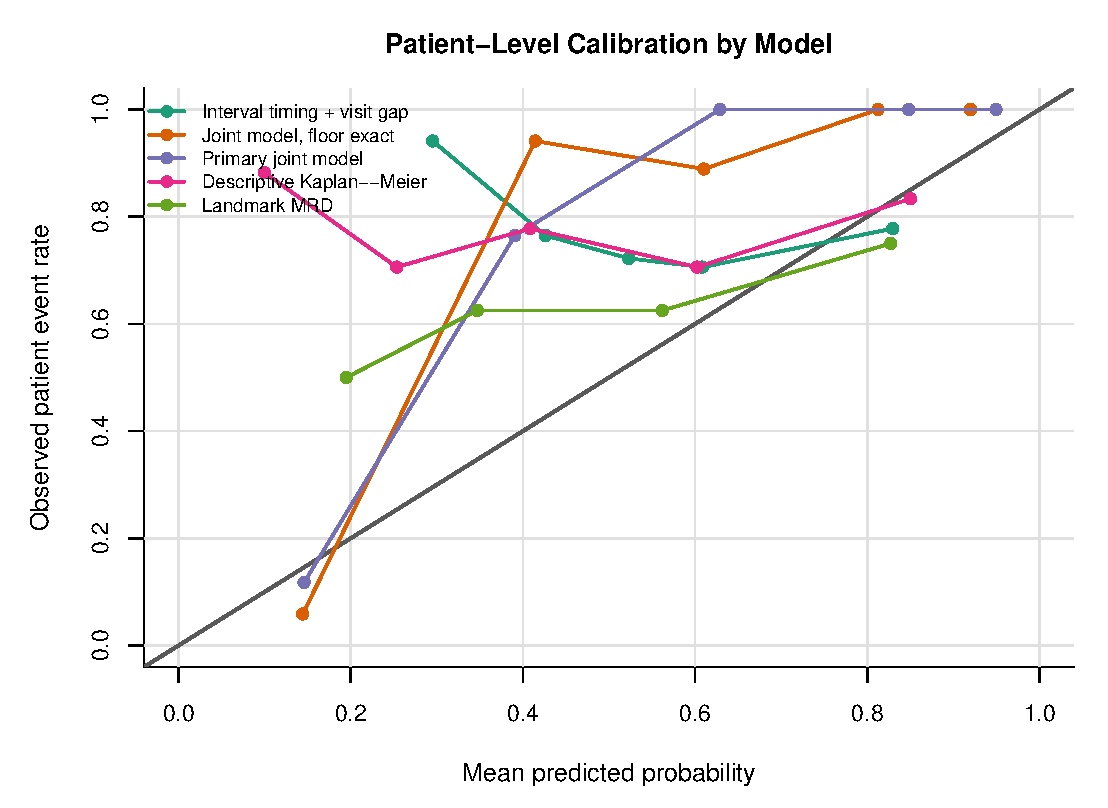
\includegraphics[width=0.82\linewidth]{figure_11_model_comparison_patient_calibration.pdf}
\caption{Patient-level observed-versus-predicted calibration across model classes. Patient-level probabilities from interval models were computed as cumulative probabilities across at-risk intervals.}
\label{fig:model-comparison-patient-calibration}
\end{figure}

For internal validation, refittable simpler models were evaluated with patient-cluster bootstrap optimism correction, preserving the clustered longitudinal and interval structure. Full bootstrap refitting of the Stan joint models was not performed because it would require repeated Bayesian refits in a cohort of 87 patients; instead, patient-cluster bootstrap summaries of the fixed posterior predictions were reported and interpreted as internal stability checks rather than full optimism correction. This distinction is important for peer review and supports cautious wording: the joint model is justified by clinical coherence, interval-aware endpoint handling, and principled assay-floor likelihood specification, but external validation remains necessary before clinical decision use.

